\documentclass[11.5pt,aspectratio=169]{beamer}
\usepackage{amsmath,amsfonts,amssymb}
\usepackage{multicol}
\usepackage{graphicx}
\usepackage{booktabs}
\usepackage{array}
\usepackage{ragged2e}
\usepackage{xcolor}
\usepackage{hyperref}

\definecolor{venetianred}{rgb}{0.78, 0.03, 0.08}
\definecolor{sacramentostategreen}{rgb}{0.0, 0.34, 0.25}
\definecolor{themeBlue}{rgb}{0.3058, 0.4745, 0.5372}
\definecolor{themeRed}{rgb}{0.6627, 0.0039, 0.1058}
\definecolor{themeYellow}{rgb}{0.8941, 0.6588, 0.1490}
\definecolor{themeLightyellow}{rgb}{0.8627, 0.8392, 0.6980}
\definecolor{softgray}{RGB}{90,90,90}

\usetheme[progressbar=frametitle]{metropolis}
\usefonttheme{metropolis}
\usecolortheme{spruce}
\setbeamercolor{background canvas}{bg=white}
\setbeamercolor{title}{fg=venetianred,bg=white}
\setbeamercolor{frametitle}{fg=venetianred,bg=white}
\setbeamercolor{normal text}{fg=black,bg=white}
\setbeamercolor{block title}{fg=white,bg=sacramentostategreen}
\setbeamercolor{block body}{fg=black,bg=themeLightyellow!40}
\setbeamercolor{itemize item}{fg=venetianred}
\setbeamercolor{itemize subitem}{fg=venetianred}
\setbeamercolor{enumerate item}{fg=venetianred}
\setbeamerfont{frametitle}{size=\Large,series=\scshape}
\setbeamerfont{title}{size=\Large,series=\scshape,family=\rmfamily}
\setbeamerfont{subtitle}{family=\rmfamily}
\setbeamertemplate{navigation symbols}{}
\defbeamertemplate{footline}{centered page number}{%
  \hspace*{\fill}%
  \usebeamercolor[fg]{page number in head/foot}%
  \usebeamerfont{page number in head/foot}%
  \insertpagenumber\,/\,\insertpresentationendpage%
  \hspace*{\fill}\vskip2pt%
}
\setbeamertemplate{footline}[centered page number]
\setbeamertemplate{itemize item}{\textcolor{venetianred}{--}}
\setbeamertemplate{itemize subitem}{\textcolor{venetianred}{-}}
\setbeamertemplate{blocks}[rounded][shadow=false]
\setbeamercovered{transparent=5}
\hypersetup{pdfpagemode=FullScreen}
\metroset{block=fill}

\title{Replication in Economics Research Basics}
\subtitle{Replication 101}
\author{}
\date{}

\newcommand{\slsource}[1]{\vspace{0.3em}{\tiny\color{softgray}Source: #1\par}}
\newcommand{\tight}{\setlength{\itemsep}{0.5em}}

\begin{document}

{%
\usebackgroundtemplate{%
  \parbox[r][0.47\paperheight][r]{\paperwidth}{%
    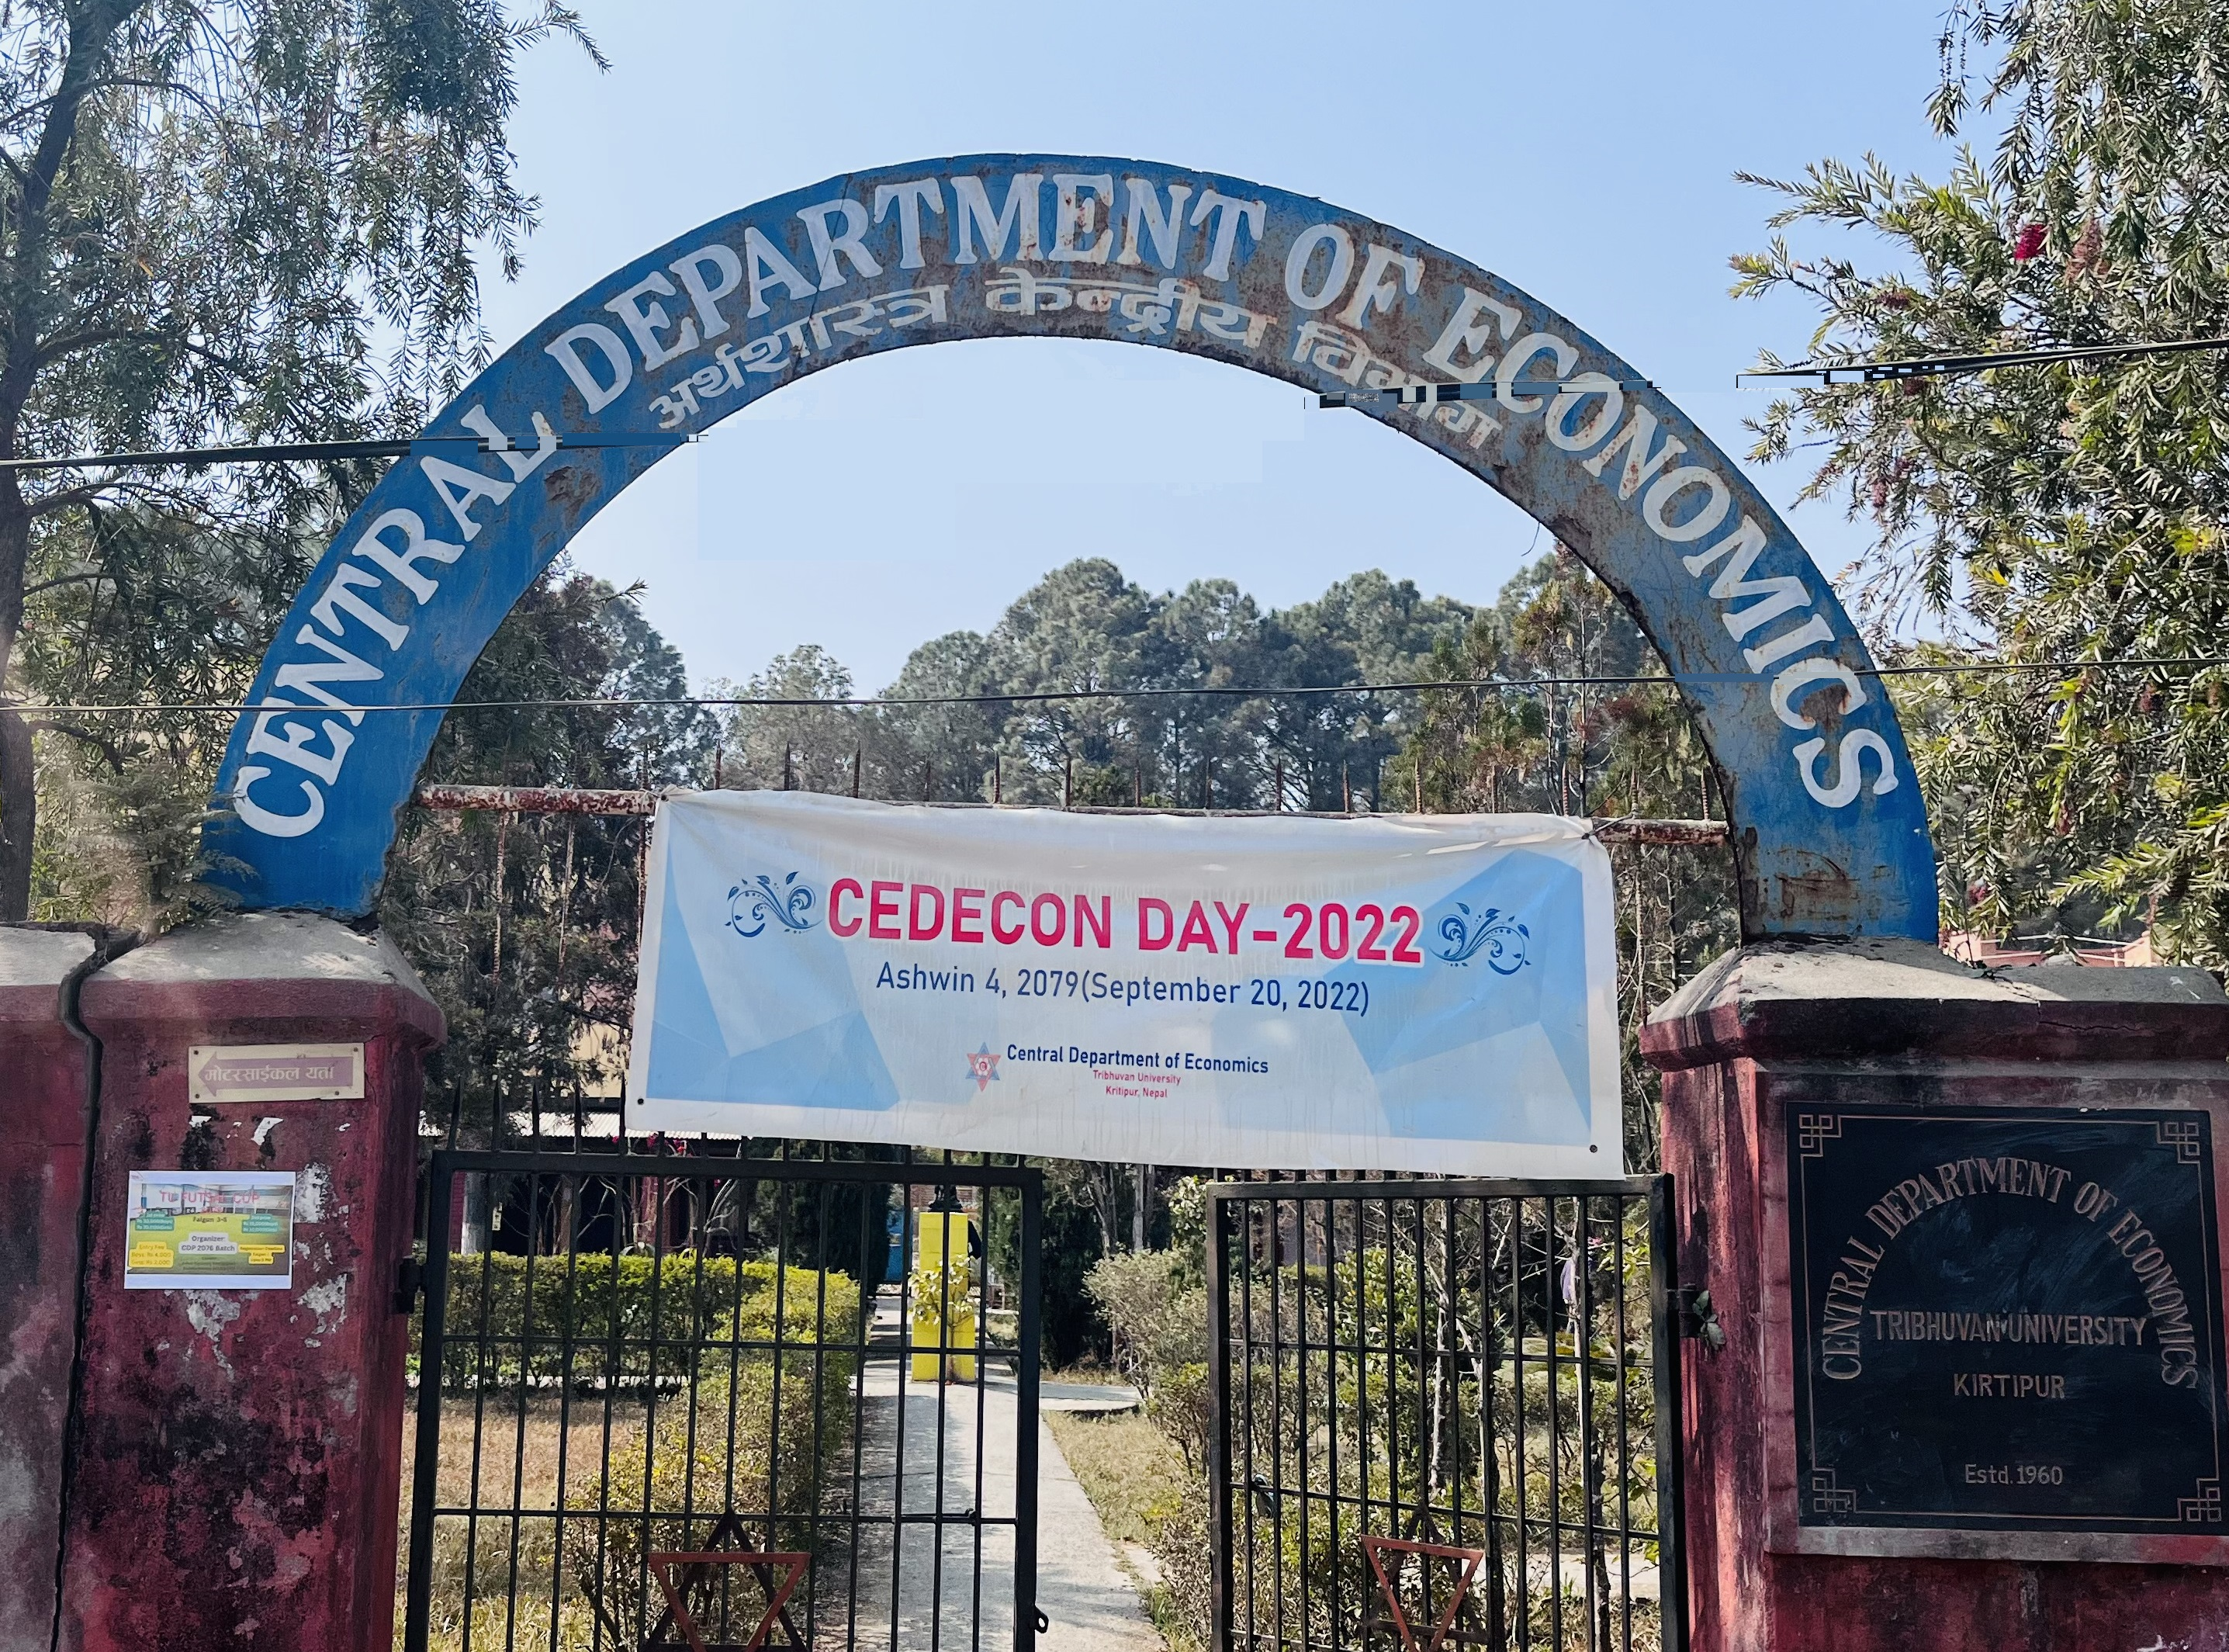
\includegraphics[height=4.3cm,keepaspectratio]{assets/board.jpg}%
    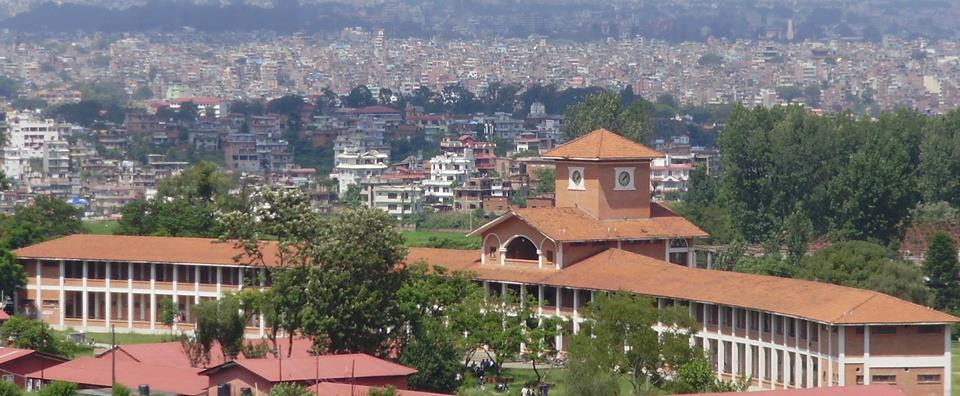
\includegraphics[height=4.3cm,keepaspectratio]{assets/arts_building.jpg}%
  }%
}
\begin{frame}[plain]
  \parbox[r][0.55\paperheight][r]{.9\paperwidth}{
  \begingroup \fontfamily{lmr}\selectfont{\LARGE\color{venetianred}{Replication in Economics\\Research Basics}}
    \endgroup}\\
  \selectfont{\vspace{.5cm}\small
    Replication 101\\
    Practical notes on replication packages, reproducibility\\
%    and journal expectations in economics\\
    }

  \parbox[r][0.22\paperheight][r]{\paperwidth}{
  \hspace{.438\paperwidth}
  
\includegraphics[height=1.2cm,keepaspectratio]{assets/TU_logo.png}
  
\includegraphics[height=1.2cm,keepaspectratio]{assets/cedecon.png}
  }
\end{frame}
}

{%
\usebackgroundtemplate{%
  \parbox[t][0.99\paperheight][r]{\paperwidth}{%
    \hspace{0.7\paperwidth}%
    
\includegraphics[height=0.7cm,keepaspectratio]{assets/TU_logo.png}%
    
\includegraphics[height=0.7cm,keepaspectratio]{assets/cedecon.png}%
  }%
}

\begin{frame}[plain]
  \centering
  \begingroup \fontfamily{lmr}\selectfont{\Large\color{venetianred}{Replication in Economics Research Basics}}\\
  \endgroup

  \vspace{0.5cm}
  {\color{sacramentostategreen}\line(1,0){290}}\\
  \selectfont{\footnotesize
    \textit{Focus:} why replication packages matter\\
    and how to build a package that another researcher can actually run.}
\end{frame}

\addtocounter{page}{-1}

\begin{frame}[t]{Why replication packages matter}
\vspace{2pt}
\begin{itemize}\tight
  \item A replication package is the bundle of data, code, documentation, and computing instructions that allows another researcher to reproduce the published results.
  \item In economics, replication matters for \textcolor{themeRed}{transparency}, \textcolor{themeBlue}{verification}, and \textcolor{sacramentostategreen}{reuse}.
  \item A well-prepared package reduces ambiguity about data construction, estimation choices, and the path from raw inputs to final tables and figures.
  \item It also turns a paper into something that can be checked, learned from, and extended by others.
\end{itemize}
\slsource{Hamermesh (2007); AEA Data Editor reports (2019, 2024).}
\end{frame}

%\begin{frame}[t]{What journal editors increasingly expect}
%\vspace{4pt}
%\begin{itemize}\tight
%  \item Leading economics journals now require authors to submit data and code sufficient for reproducibility as a condition of publication.
%  \item The AEA Data Editor manages reproducibility checks, archives replication packages, and verifies whether submitted materials can recreate the paper's results.
%  \item The package should normally include the analysis data or access instructions, code for cleaning and estimation, a clear README, and enough documentation to map scripts to outputs.
%  \item The standard is not merely \emph{having files}; it is providing a package that an informed outsider can run successfully.
%\end{itemize}
%\slsource{AEA Papers and Proceedings accepted-article guidance; Report of the AEA Data Editor (2019, 2024).}
%\end{frame}

\begin{frame}[t]{The key principle: computational empathy}
\vspace{2pt}
\begin{columns}[T]
\begin{column}{0.52\linewidth}
\begin{block}{Core idea}
\justifying
Write the package for a careful graduate student working on a clean machine, not for the author who already knows the project history.
\end{block}
\end{column}
\begin{column}{0.46\linewidth}
\begin{block}{Ask yourself}
\justifying
Could someone else run this without my laptop, local folders, or undocumented manual steps?
\end{block}
\end{column}
\end{columns}

\vspace{0.45em}
\begin{columns}[T]
\begin{column}{0.48\linewidth}
\textcolor{venetianred}{Do:}
\begin{itemize}\tight
%  \item use relative paths
  \item provide one master run file
  \item pin software versions where important
  \item explain restricted-data branches honestly
\end{itemize}
\end{column}
\begin{column}{0.48\linewidth}
\textcolor{venetianred}{Avoid:}
\begin{itemize}\tight
  \item manual clicking and hand edits
  \item hidden preprocessing
  \item missing dependencies
  \item output folders that do not reproduce cleanly
\end{itemize}
\end{column}
\end{columns}
\slsource{AEA Data Editor practical guidance on preparing files for verification.}
\end{frame}

% Reset logo for a specific frame
\usebackgroundtemplate{}
\begin{frame}[t]{A practical structure for a replication package}
\small
\begin{table}
\centering
\begin{tabular}{p{0.26\textwidth}p{0.66\textwidth}}
\toprule
\textbf{Folder / file} & \textbf{What it should do} \\
\midrule
\texttt{README} & Explain software, runtime, execution order, data availability, and table/figure mapping \\
\texttt{data/raw/} & Store original data or document how restricted/proprietary data are accessed \\
\texttt{data/analysis/} & Hold cleaned or constructed datasets used in estimation \\
\texttt{code/} & Include scripts for cleaning, estimation, diagnostic tests, and figures \\
\texttt{run\_all.do} / \texttt{main.R} & Provide a single entry point for rerunning core results \\
\texttt{results/} & Save generated tables, figures, logs, and diagnostics \\
\bottomrule
\end{tabular}
\end{table}
%\vspace{0.10em}
\begin{block}{Rule of thumb}
\scriptsize
If a stranger cannot tell what to run, in what order, with which software, and what successful output should look like, the package is not ready.
\end{block}
\slsource{AEA policy guidance and editor recommendations.}
\end{frame}

% Reset logo for a specific frame
\usebackgroundtemplate{}
\begin{frame}[t]{Common failure points}
\vspace{4pt}
\begin{itemize}\tight
  \item \textcolor{themeRed}{Late assembly:} authors organize files only after acceptance.
  \item \textcolor{themeRed}{Weak README:} no runtime, software, or output map.
  \item \textcolor{themeRed}{Confidential-data confusion:} missing explanation of what can and cannot be shared.
  \item \textcolor{themeRed}{Code rot:} scripts accumulated across multiple machines no longer run from scratch.
  \item \textcolor{themeRed}{Hidden workflow steps:} manual preprocessing exists outside the documented pipeline.
\end{itemize}
\vspace{0.4em}
\begin{block}{Editor-side implication}
\scriptsize
A package may seem complete to the author and still fail verification because the files do not reproduce the claimed results on an external machine.
\end{block}
\slsource{Arne Seibold's Open Science Day slides; AEA Data Editor reports.}
\end{frame}

\begin{frame}[t]{Replication 101 workflow for students}
\vspace{2pt}
\begin{enumerate}\tight
  \item Choose a paper with feasible data access and manageable software requirements.
  \item Map the pipeline from raw data to cleaned data, estimates, and final exhibits.
  \item Reproduce the headline tables and figures before attempting extensions.
  \item Record every deviation from the published workflow.
  \item Re-run the full pipeline from a clean session.
  \item Write a README for another person, not for your future self.
  \item Archive outputs and logs so failures can be diagnosed.
\end{enumerate}
\vspace{0.35em}
\begin{block}{Pedagogical value}
Replication teaches empirical design by forcing the researcher to understand data construction, coding choices, and the logic linking methods to results.
\end{block}
\slsource{Henderson and Parmeter on replication as a teaching tool; Höffler (2014).}
\end{frame}

%\begin{frame}[t]{Useful professor/editor materials to look up}
%\small
%\begin{tabular}{p{0.35\textwidth}p{0.57\textwidth}}
%\toprule
%\textbf{Material} & \textbf{Why it is useful} \\
%\midrule
%AEA Data Editor: \emph{Ten Simple Rules for Creating a Replication Package} & concise checklist from the editor's perspective \\
%AEA Data Editor reports & explains the role of reproducibility checks and common package problems \\
%Arne Seibold: \emph{Data and Replication Policies in Economics} & clear overview of journal policy trends and author-side preparation \\
%Hamermesh: \emph{Replication in Economics} & classic statement of why replication matters in the discipline \\
%Henderson and Parmeter: teaching with replication & emphasizes the training value of replication for econometrics students \\
%\bottomrule
%\end{tabular}
%\slsource{Public professor/editor materials and journal guidance pages.}
%\end{frame}

% Restore the logo for subsequent frames
\usebackgroundtemplate{%
	\parbox[t][0.99\paperheight][r]{\paperwidth}{%
		\hspace{0.7\paperwidth}%
		
\includegraphics[height=0.7cm,keepaspectratio]{assets/TU_logo.png}%
		
\includegraphics[height=0.7cm,keepaspectratio]{assets/cedecon.png}%
	}%
}
\begin{frame}[t]{Takeaway checklist}
\vspace{4pt}
\begin{itemize}\tight
  \item Can someone rerun the package without access to my personal machine?
  \item Is there one obvious command or script that reproduces the core results?
  \item Does the README explain data rights, software, runtime, and output mapping?
  \item Are restricted or proprietary components documented clearly and honestly?
  \item Did I rerun everything from scratch after cleaning folders and outputs?
\end{itemize}
\vspace{0.7em}
\centering
{\large\color{venetianred}A good replication package is not extra paperwork;}\\
{\large\color{sacramentostategreen}it is part of credible empirical research.}
\end{frame}

\begin{frame}[t]{Selected sources}
\footnotesize
\begin{itemize}\setlength{\itemsep}{0.45em}
\scriptsize
  \item American Economic Association, accepted article guidelines and Data and Code policy pages.
  \item Vilhuber, Lars. ``Report of the AEA Data Editor,'' \emph{AEA Papers and Proceedings}, 2019 and 2024.
  \item Hamermesh, Daniel S. ``Replication in Economics,'' NBER Working Paper 13026, 2007.
  \item Henderson, Daniel J., and Christopher F. Parmeter. Work on using replication to teach and understand econometrics.
  \item Seibold, Arne. Open Science Day 2023 slides on data and replication policies in economics.
  \item Tyner, A. H., Abatayo, A. L., Daley, M., Field, S., Fox, N., Haber, N. A., ... & McHugh, C. (2026). Investigating the replicability of the social and behavioural sciences. Nature, 652(8108), 143-150.
  \item Hamermesh, D.S. (2007), Viewpoint: Replication in economics. Canadian Journal of Economics/Revue canadienne d'économique, 40: 715-733. https://doi.org/10.1111/j.1365-2966.2007.00428.x
  \item Höffler, Jan H. 2017. "Replication and Economics Journal Policies." American Economic Review 107 (5): 52–55.
  DOI: 10.1257/aer.p20171032
  \item Sukhtankar, S. (2017). Replications in development economics. American Economic Review, 107(5), 32-36.
\end{itemize}
\end{frame}

}
\end{document}
